\documentclass[a4paper,10pt]{article}

\usepackage{multicol,color,graphicx,url,spconf,amsmath,algorithm,algorithmicx,algpseudocode}
\usepackage[noadjust]{cite}
\usepackage[utf8]{inputenc}
\usepackage[english]{babel}


  \title{Comparative Difference Between Dijkstra \& Bellman-Ford Algorithm}
  \name{Mir Mursalin Ankur{\small $^{1}$} \& Md. Resbi Anik{\small $^{1}$}}
  \address{{\small $^{1}$}Dept. of Computer Science \& Engineering, RUET}
  \date{\today}

\begin{document}
\maketitle

\pagenumbering{roman}
\begin{abstract}
Both Dijkstra and Bellman-Ford algorithm are used to find the shortest path between two or more nodes. They have different characteristics. Both algorithms have advantages and limitations upon each other. They are generally used in different sectors like as networking and communication, transportation, system analysis, business sector etc. Here we will discuss about performances of both algorithms like as time complexity, space complexity and negative cycle checking. To compare the algorithms we will use C++ programming language.
   \end{abstract}

\section{Introduction}
In mathematics graph theory is the study of graphs, which are mathematical structures used to model pairwise relations between objects. A graph in this context is made up of vertices, nodes, or points which are connected by edges, arcs, or lines.\\
In computer science, a graph is an abstract data type that is meant to implement the undirected graph and directed graph concepts from mathematics. These pairs are known as edges, arcs, or lines for an undirected graph and as arrows, directed edges, directed arcs, or directed lines for a directed graph.~\cite{re1}
\\\\
In general sense we can divide graph into two parts. One of them is weighted graph and another is un-weighted graph.
\\
In graph theory, the shortest path problem is the problem of finding a path between two vertices (or nodes) in a graph such that the sum of the weights of its constituent edges is minimized.~\cite{re2}
\\\\
Shortest path problem means the problem of finding the shortest path in graph from one vertex to another. "Shortest" may be least number of edges, least total weight etc. There are different kinds of shortest path algorithms:\\
\begin{enumerate}
  \item Single source shortest path Algorithm
  \item Single destination shortest path Algorithm
  \item All pair shortest path Algorithm
\end{enumerate}
In single source shortest path algorithm we will consider both directed and undirected graphs. In graph, all edges must have non-negative weights and graph must be connected. In this paper , we are comparing time, space, cycle checking and other criteria of single source Dijkstra and Bellman-Ford algorithm. For comparing complexity we are taking Big O notation as standard. Here cycle checking means capability of negative cycle detecting between both algorithms.
\\\\
The term Negative cycle means a cycle with weights that sum to a negative number in a graph.~\cite{re3}\\
\begin{figure}[h]
 \centering
  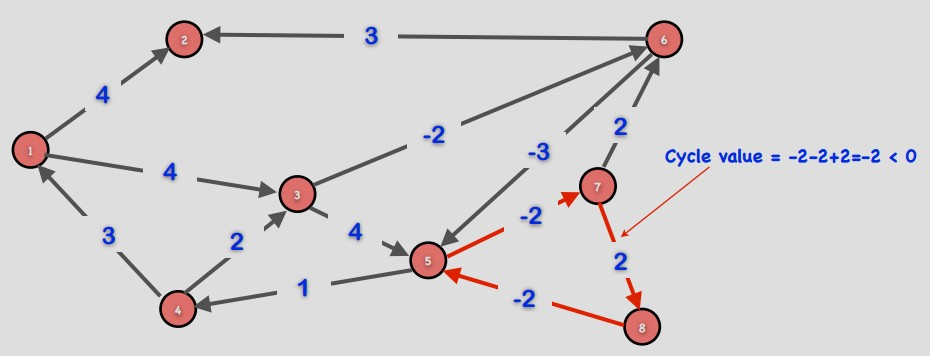
\includegraphics[width=2.5in]{negfiga.png}
    \caption{Sample Graph with negative cycle}
  \label{fig:neg fig a}
\end{figure}
\\\\
\textbf{Why the comparison is needed between Dijkstra and Bellman-Ford Algorithm:}\\\\
Bellman-Ford algorithm is a single source shortest path algorithm, which allows for negative edge weight and can detect negative cycles in a graph.
Dijkstra algorithm is also another single-source shortest path algorithm. However, the weight of all the edges must be non-negative. A comparative discussion between both algorithm will lead us to finding better algorithm for real life problem.
\\
\section{General discussion on Dijkstra and Bellman-Ford algorithm}
Primary deliberation of both algorithms are given beneath :-\
\subsection{Dijkstra Algorithm}
Dijkstra algorithm is the method of choice for finding shortest paths in an edge-weighted or vertex-weighted graph. Given a particular start vertex s, it finds the shortest path from s to every other vertex in the graph.
\\\\
\textbf{Psudocode: Shortest Path - Dijkstra(G, s)~\cite{re4}}
\begin{algorithm}
    \caption{Dijkstra Algorithm}
    \label{dij}
    \begin{algorithmic}[1]
        \Procedure{Dijkstra}{$G,s$}
        \\
        \ForAll{$v\in G$} \State $dis[v]:=\infty$ \State $previous[v]:=undefined$\EndFor
        \State $dis[s]:=0$ \State Q := the set of all nodes in Graph
        \While{Q != empty} \State u := node in Q with smallest $dist[]$ \State remove u from Q \EndWhile
        \ForAll{neighbor v of u:}
            \State $alt := dist[u] + dist\_between(u, v)$
            \If{$alt < dist[v]$} \State $dist[v] := alt$ \State $previous[v] := u$ \EndIf
        \EndFor
        \State  return $previous[ ]$

        \EndProcedure
        \\\\
        \Comment{$G=Graph$,$s=source$,$v=vertex$,$dis=distance$}
    \end{algorithmic}
\end{algorithm}
\\
\textbf{Dijkstra Implementation Technique:}\\\\
Detailed steps used in Dijkstra’s algorithm to find the shortest path from a single source vertex to all other vertices in the given graph.
\begin{enumerate}
  \item Create a set sptSet (s=shortest p=path t=tree set) that keeps track of vertices included in shortest path tree, i.e., whose minimum distance from source is calculated and finalized. Initially, this set is empty.
  \item  Assign a distance value to all vertices in the input graph. Initialize all distance values as INFINITE. Assign distance value as 0 for the source vertex so that it is picked first.
  \item While sptSet doesn’t include all vertices
  \begin{enumerate}
    \item Pick a vertex u which is not there in sptSet and has minimum distance value.
    \item Include u to sptSet.
    \item Update distance value of all adjacent vertices of u. To update the distance values, iterate through all adjacent vertices. For every adjacent vertex v, if sum of distance value of u (from source) and weight of edge u-v, is less than the distance value of v, then update the distance value of v.
  \end{enumerate}
\end{enumerate}
\textbf{Example of Dijkstra Algorithm:}\\\\

 \begin{figure}[h]
 \centering
  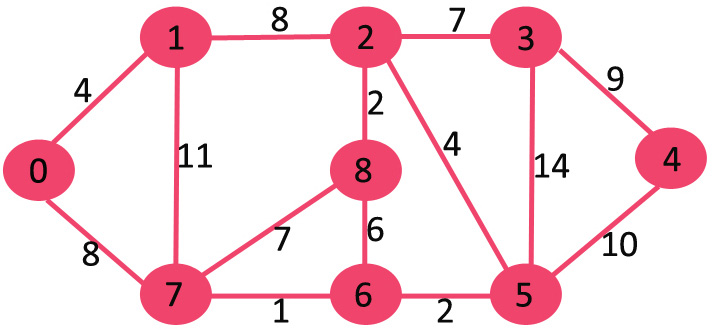
\includegraphics[width=1.5in]{dijfiga.png}
    \caption{A Weighted Graph~\cite{re5}}
  \label{fig:dij fig a}
\end{figure}
The set sptSet is initially empty and distances assigned to source vertex are 0 and else other vertices are $\infty$.\\
\hfill
 Now there should pick the vertex having minimum distance value. The vertex 0 is picked, include it in sptSet. SptSet becomes {0} and only one element is inserted into set.\\
Now update distance values of its adjacent vertices.0’s adjacent vertices are 1 and 7. The distance values of 1 is updated as 4 and 7 is updated as 8.~\cite{re5}\\
 \begin{figure}[h]
 \centering
  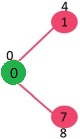
\includegraphics[width=0.5in]{dijfigb.png}
    \caption{Sub Graph of Fig.2~\cite{re5}}
  \label{fig:dij fig b}
\end{figure}
The subgraph in Fig.3 shows vertices and their distance values as indicated at the top of the vertices,. The vertices included in SPT are shown in another color. Here it is green.\\
\begin{figure}[h]
 \centering
  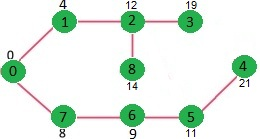
\includegraphics[width=2.0in]{dijfigf.png}
    \caption{Shortest Path according to Dijkstra Algorithm~\cite{re5}}
  \label{fig:dij fig f}
\end{figure}
\\Now it should pick the vertex having minimum distance value and not already included in the set of sptSet. This process repeats this steps until sptSet doesn’t include all vertices of given graph which shortest path is needed. The result is showed in fig 4.

\subsection{Bellman-Ford Algorithm}
Bellman–Ford is also a shortest path algorithm. In this algorithm, an approximation to the correct distance is gradually replaced by more accurate values until eventually reaching the optimum solution.\\\\
\textbf{Pseudocode: Shortest Path - BELLMAN-FORD(G,w,s)~\cite{re6}}
\begin{algorithm}
    \caption{Bellman-Ford Algorithm}
    \label{bel}
    \begin{algorithmic}[1]
        \Procedure{Bellman-Ford}{$G,w,s$}
        \\
        \For{$i = 1$ to $|G.V|-1$}
            \ForAll{edge $(u,v)\in G.E$} \Call{relax}{u,v,w}\EndFor
        \EndFor
        \ForAll{edge $(u,v)\in G.E$}
        \If{$v.d > u.d + w(u,v)$} \State return false \Else \State return false \EndIf
        \EndFor
        \EndProcedure
        \\\\
        \Comment{$G=Graph$, $w=weight$, $s=source$, $V=Vertex$}\\
        \Comment{$E=Edge$, $d=distance$, $(u,v)=node$}
    \end{algorithmic}
\end{algorithm}
\\\\
\textbf{Bellman-Ford Implementation Technique:}\\
\begin{enumerate}
  \item This step initializes distances from source to all vertices as infinite and distance to source itself as 0. Create an array dist[] of size $|V|$ with all values as infinite except dist[src] where src is source vertex.
  \item This step calculates shortest distances. Do following $|V|-1$ times where $|V|$ is the number of vertices in given graph. Do following for each edge u-v.\\
         \hfill If $dist[v] > dist[u] + weight$ of edge uv, then update dist[v].\\
             \hfill \hfill $dist[v] = dist[u] + weight$ of edge u-v.

  \item This step reports if there is a negative weight cycle in graph. Do following for each edge u-v.
If $dist[v] > dist[u] + weight$ of edge uv, then “Graph contains negative weight cycle”.\\\\
\hfill The idea of step 3 is, step 2 guarantees shortest distances if graph doesn’t contain negative weight cycle. If we iterate through all edges one more time and get a shorter path for any vertex, then there is a negative weight cycle.\\
\end{enumerate}

\textbf{Example of Bellman-Ford Algorithm:}\\

\begin{figure}[h]
 \centering
  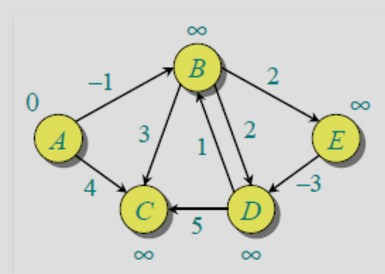
\includegraphics[width=1.5in]{belfigd.png}
    \caption{Negative Cycle Checking With Bellman-Ford Algorithm~\cite{re7}}
  \label{fig:bel fig d}
\end{figure}
\vspace{.5 cm} Let the given source vertex be 0. Initialize all distances as infinite, except the distance to source itself. Total number of vertices in the graph is 5, so all edges must be processed 4 times.\\

Let all edges are processed in following order: (B,E), (D,B), (B,D), (A,B), (A,C), (D,C), (B,C), (E,D). We get following distances when all edges are processed first time. The first row in shows initial distances.\\
\begin{figure}[h]
 \centering
  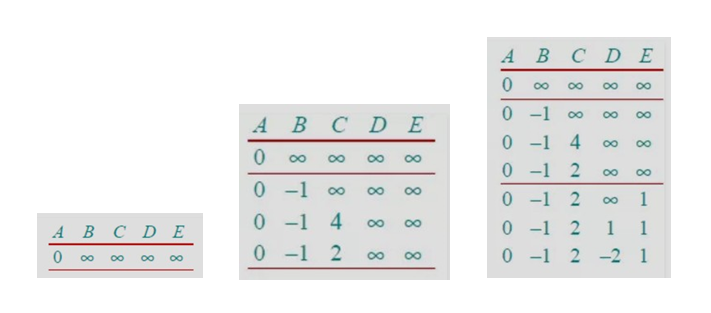
\includegraphics[width=2.5in]{belfige.png}
    \caption{Sequential iteration of Fig. 5 implementing Bellman-Ford Algorithm~\cite{re7}}
  \label{fig:bel fig e}
\end{figure}
The first iteration guarantees to give all shortest paths which are at most 1 edge long. We get following distances when all edges are processed second time.\\\\
The second iteration guarantees to give all shortest paths which are at most 2 edges long. The distances are minimized after the second iteration, so third and fourth iterations don’t update the distances. The last row in Fig.6 shows final values.
\\\\
\section{Comparison}
\begin{figure}[h]
 \centering
  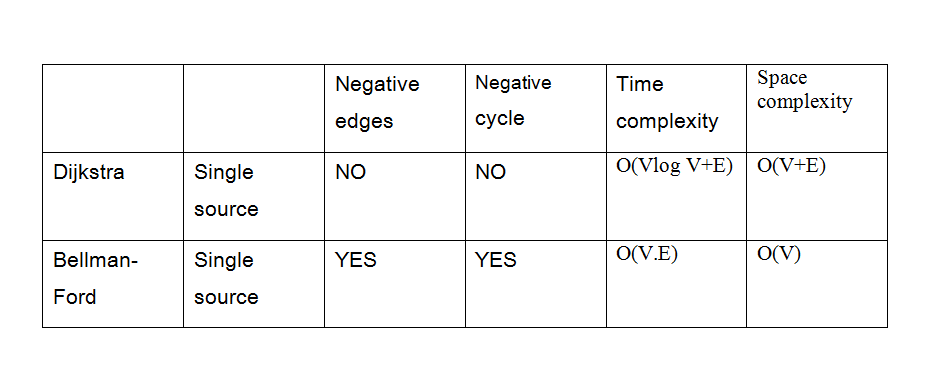
\includegraphics[width=3.0in]{comfigc.png}
    \caption{Comparative Difference Table~\cite{re8}}
  \label{fig:com fig c}
\end{figure}

\textbf{Complexity :}\\\\
Computational complexity is the study of the inherent limits of efficient computation measured in terms of time, space, and other resources such as randomness. Complexity between Dijkstra and Bellman-Ford algorithm on different aspect is shown in Fig. 7.\\

\begin{figure}[h]
 \centering
  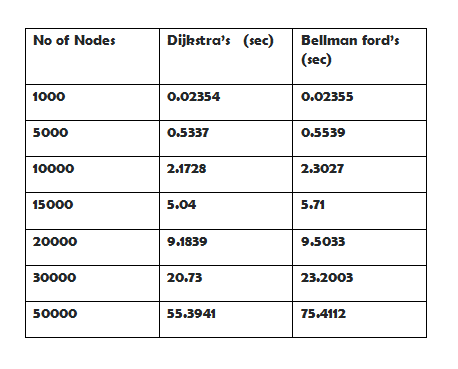
\includegraphics[width=3.0in]{comfigd.png}
    \caption{Chart of experimental values}
  \label{fig:com fig d}
\end{figure}

\textbf{Experimental value : }\\\\
We have calculated some experimental values by using C++ programming language. A PC with intel core i3 CPU of $3^{rd}$ generation and 4GB DDR3 RAM configuration show experimental value in Fig. 8. and Fig. 9.\\\\
\begin{figure}[h]
 \centering
  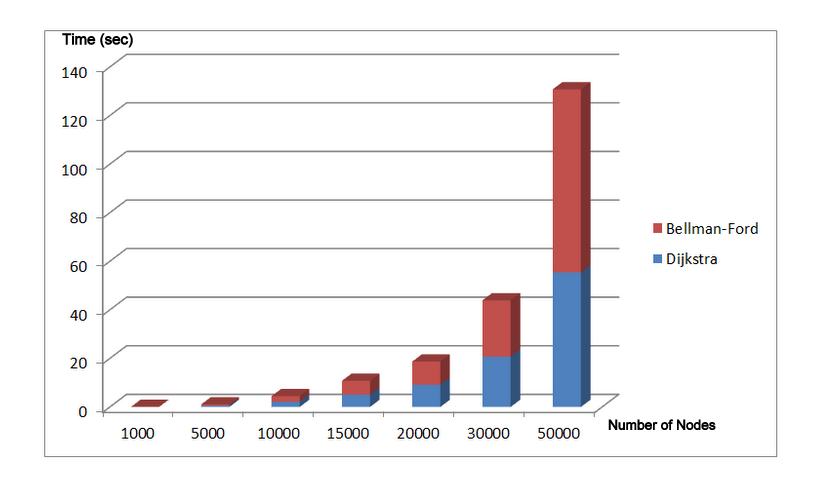
\includegraphics[width=3.0in]{comfige.png}
    \caption{Histogram according to Fig. 8 showing comparative time complexity}
  \label{fig:com fig e}
\end{figure}\\
\section{Conclusion:}
After studying these two algorithms we conclude that Dijkstra algorithm is faster than Bellman-Ford algorithm. Though at the perspective of negative cycle checking Bellman-Ford is better. But time complexity of Bellman-Ford algorithm is larger than Dijkstra algorithm for finding shortest path. Which is a important factor in real life graph based problem like GIS (Geographic Information System), networking, pattern finding etc. So, Dijkstra algorithm is widely used in real time application. For better and faster performance in larger system Dijkstra is automatic choice between Dijkstra and Bellman-Ford algorithm.\\

\begin{thebibliography}{10}

\vspace{.1cm}

\bibitem{re1}
\newblock \url{https://en.wikipedia.org}

\bibitem{re2}
Introduction to Algorithms by Thomas H. Corman

\bibitem{re3}
\newblock \url{http://algo.epfl.ch}

\bibitem{re4}
\newblock \url{http://www.gitta.info}

\bibitem{re5}
\newblock \url{http://www.geeksforgeeks.org}

\bibitem{re6}
The Algorithm Design Manual by Steve S. Skiena

\bibitem{re7}
\newblock \url{http://www.shafaetsplanet.com}


\bibitem{re8}
\newblock \url{http://www.stackoverflow.com}


\end{thebibliography}
\end{document} 